%%% 関西大学 総合情報学部 松下ゼミ 進捗報告 TeXテンプレート Ver 1.1 (2011/12/04) %%%
\documentclass{matsushita-zemi}
\usepackage[dvipdfmx]{graphicx}
\usepackage{comment}
\graphicspath{{./fig/}}

%%% タイトル (長くなる場合は¥¥で適宜改行すること)%%%
\title{動向情報の可視化手法}

%%% 氏名 (姓・名の間は半角スペース) %%%
\author{内藤 峻}

\begin{document}
\maketitle

%%% 以下、本文 %%%
\section*{概要}
\label{abstract}
ネットワーク上には多様な種類の情報が存在しており、それらをユーザの要求に応じて適応的にまとめ上げる技術が渇望されている。その一つとして、テキストなどの言語情報と統計データ等の数値情報の相補的な利用に関する研究が行われている。その一環として、本研究では言語情報と数値情報が密接な関係にある株価などの動向情報に着目しそれらを統一的な枠組みで可視化する手法を提案する。株価などの統計情報の場合、その正確な値を知るには数値情報が適切であるのに対して、変動の大局的な理解や背景となる事象の把握には言語情報が適している。そこで、これらを一つのグラフ上に提示し、その情報源に対話的にアクセスできるようにする。\cite{Elucignage}

\section{はじめに}
\label{background}
%電子化が普及している話
%それらの情報を利用して意思決定や問題解決に役立てられている話
%しかし、情報は膨大になっている、時間にともなって更に増加を続けている話
%既存の検索技術ではユーザの要求に答えることができない
%それらをまとめる技術が求められている話
%しかし、情報には様々な種類がある話
%本提案では数値情報(統計データ)と言語情報(新聞記事)に着目した話
近年、様々な情報が電子化されネットワーク上に蓄積されている。それに伴い、これらの情報を利用して意思決定や問題解決に役立てる試みがなされている。しかし、蓄積された情報は膨大であるうえ、時間の経過に伴って更に増加を続けている。そのため、"情報の在処を見つける"ことを主眼とした検索技術ではユーザの要求に十分に応えることができず、ユーザの関心や興味に合致する情報に直感的かつ簡便にアクセスするための技術、言うなれば"情報の理解を助ける技術が渇望されている。\cite{information_compilation}\cite{Elucignage-jsai}。
%情報にはテキスト、画像、音声、動画と様々な種類がある。
このような要求に答える技術のひとつとして、本提案では統計データ等の数値情報と新聞記事等の言語情報を相補的に用いて編纂し、ユーザの情報アクセス行為を容易にする技術の実現をめざす。

ネットワーク上にはテキストや統計データ、音声、画像動画など様々な種類の情報が存在している。将来的にはそれらの情報全てを対象とし、状況や目的に応じて取捨選択やモード変換を行い、適切な形態で組み合わせてユーザに提供することが望まれるが、現在の技術レベルではその実現は容易ではない。そこで本研究では、まず時間的変動を伴う統計データ(時系列数値情報)とそれに関連する記事(言語情報)を対象とし、ユーザがそれらの情報にアクセスしたり、その概要を把握したりする際の支援となる可視化手法について議論する。

本稿では、まず、先行研究について述べる。次に、デザイン指針を説明し、その後、先行研究を示す。

\section{先行研究}
\label{relatedworks} 
動向情報を可視化する枠組みとして、山本らの可視化システム\cite{Tagged_corpus}や松下らのSTEND\cite{STEND}、高間らの地震情報可視化システム\cite{SpaceTrendInformation}などがある。

山本らは、動向情報の変化要因に関する重要語を注釈としてグラフに表示する方法を提案している(図\ref{system})\cite{タグ付きコーパス}。要因の抽出では、動向情報が記載された新聞記事と文章の類似度が高い新聞記事を要因としている。また、要因とされた新聞記事からのキーワード抽出は、1月分の新聞記事を1ドキュメントとみなしたTF・IDF値に基づき行っている。動向情報とその要因の表示方法に関するアンケート調査からは、ユーザが動向情報に関する要因を知りたいことは、動向情報を示したグラフ中の変化が大きい部分とその前後、最大位置と最小位置、及び最初と最後の3つに分類できることが分かったと述べられている。また、要因の表示方法としては、1ウィンドウに3つ程度のトピックを簡潔に示したものや、要因をタイトルやキーワードとともに表示すれば良いことが分かったと述べられている。
\begin{figure}[tb]
  \begin{center}
   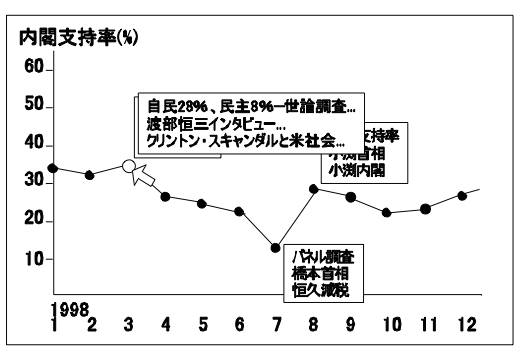
\includegraphics[width=8cm,bb=0 0 521 356]{tagu.PNG}
  \end{center}
 \caption{山本らのシステムの出力例}
 \label{system}
\end{figure}
%%%この方法は本稿の提案方法と問題意識が近く、特に情報提示に関しては参考になる点も多い。しかし、その情報提示がユーザとのインタラクションにおいてどのように作用し適応していくかについては、現状ではあまり深く検討されていない。本提案はユーザのインタラクションに基づく適応的情報提示に大きな関心があり、この点でこれらの方法と方向性が異なる。%%%

松下らは、グラフ概形を示唆するシステムSTENDを提案している\cite{STEND}。STENDは時系列数値情報を扱わず、新聞記事のテキストデータのみから取得可能な数値情報と定性情報に着目してグラフ描画を試みたものである(図\ref{STEND})。テキスト中の「昨年10月より約40%の下落になっている」「前年同月に比べて5ドル上昇した」等の比較表現や「安定傾向にあった」「10月をピークに下落している」等の定性表現から情報を抽出している。情報提示では、統計グラフを用いず数種類の点や短形、形状の異なる幾つかの矢印記号を組み合わせることでその代替を試みている。

%%%松下らは、グラフ概形を示唆するシステムSTENDを提案している。STENDは時系列数値情報を扱わず、新聞記事のテキストデータのみから取得可能な数値情報と定性情報に着目してグラフ描画を試みたものであり、本提案とは力点が異なる。テキスト中の「昨年10月より約40%の下落になっている」「前年同月に比べて5ドル上昇した」等の比較表現や「安定傾向にあった」「10月をピークに下落している」等の定性表現から情報を抽出している。情報提示では、統計グラフを用いず数種類の点や短形、形状の異なる幾つかの矢印記号を組み合わせることでその代替を試みている。
\begin{figure}[tb]
  \begin{center}
   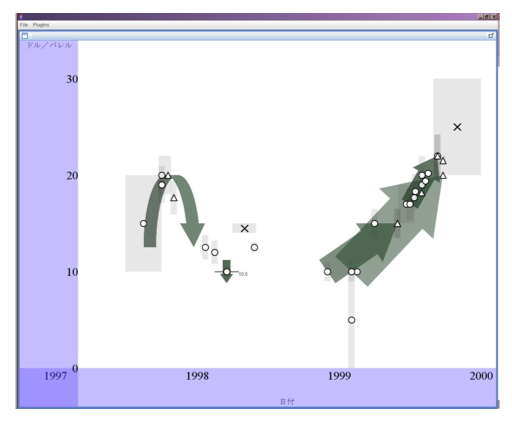
\includegraphics[width=8cm,bb=0 0 512 422]{STEND.PNG}
  \end{center}
 \caption{STENDの描画例}
 \label{STEND}
\end{figure}

\section{デザイン指針}
%目的をどのように達成するのかという話
%どのような機能が必要なのか?何故必要なのか?
%シナリオに基づいた話
%必要な機能な整理
%シナリオを載っけるのもあり
%言語情報と数値情報を扱う話
%それらをどのように見せるか、どのようなインタラクションを想定するのかという話
%変化の実験の論文を引用
まず、本研究で扱う数値情報と言語情報の特徴について述べる。
統計情報等の数値情報は正確である。
変わって、言語情報はあいまいであるものの、その時点の背景等を理解することができる。
本研究では、数値情報には統計DBを、言語情報には新聞記事を用いて、ユーザの効率的なアクセスを促すシステムを提案する。
ユーザの効率的なアクセスを支援するためにはユーザのふるまいを想定をする必要がある。
ユーザはグラフを見て、そのときの変化における要因や背景を知りたいと思う。そこで、本提案ではユーザの興味や関心を想定したインタラクションを考える。
ユーザはグラフの変曲点になる部分に興味を持つ。
また、そこで、要因と背景を知りたいと思う。
以下の様なシナリオを想定している。


\section{Elucignage プロトタイプシステム}
\subsection{概要}
%書き直し、もう少し詳しく述べられるはず
ユーザは統計グラフの外観を理解するだけでなく、興味を持った箇所についてどのようなことが述べられているかをその要因となる記事にアクセスすることで参照できる。そのため、ユーザの関心がある動向情報を時系列数値情報を用いて統計グラフとして描画し、そのグラフの要因となる記事をその内容に適したアイコンの形式で提示する方法を採用する。このアイコンは要因となる記事のアクセスを可能にする。また、記事の一部を画面の一部に表示し、そこからグラフのどの部分に該当しているかを示す機能を備える。これにより、要因となる記事がグラフのどの部分で記述されたものであるかを確認できる。
\subsection{実装}
現段階の実装に関して述べる。
検索ボックス
記事リストパネル
グラフパネル
コントロールパネル

\section{おわりに}
本稿では、動向情報の可視化手法について考察した。先行研究として山本らの可視化システムや松下らのSTEND、蓮井らのグラフ型インタフェース、加藤らの視覚オブジェクトを報告した。続いて、卒業研究への展望を示した。

%%% 参考文献 %%%
\bibliographystyle{ipsjsort}
\bibliography{reference}

\end{document}